\section{Rest-Endpoints}
\setauthor{Oliver Sugic}

Wichtig war es, die Schnittstellen so zu implementieren, das Sie sowohl GET Requests für das anzeigen von Reisen und Aktivitäten, als auch POST Requests für das Erstellen von Reisen.
Jede Entität hat eine CRUD Funktionalität implementiertet. Im Quarkus Swagger kann man sich die Schnittstellen anschauen:

\begin{figure}[h]
    \centering
    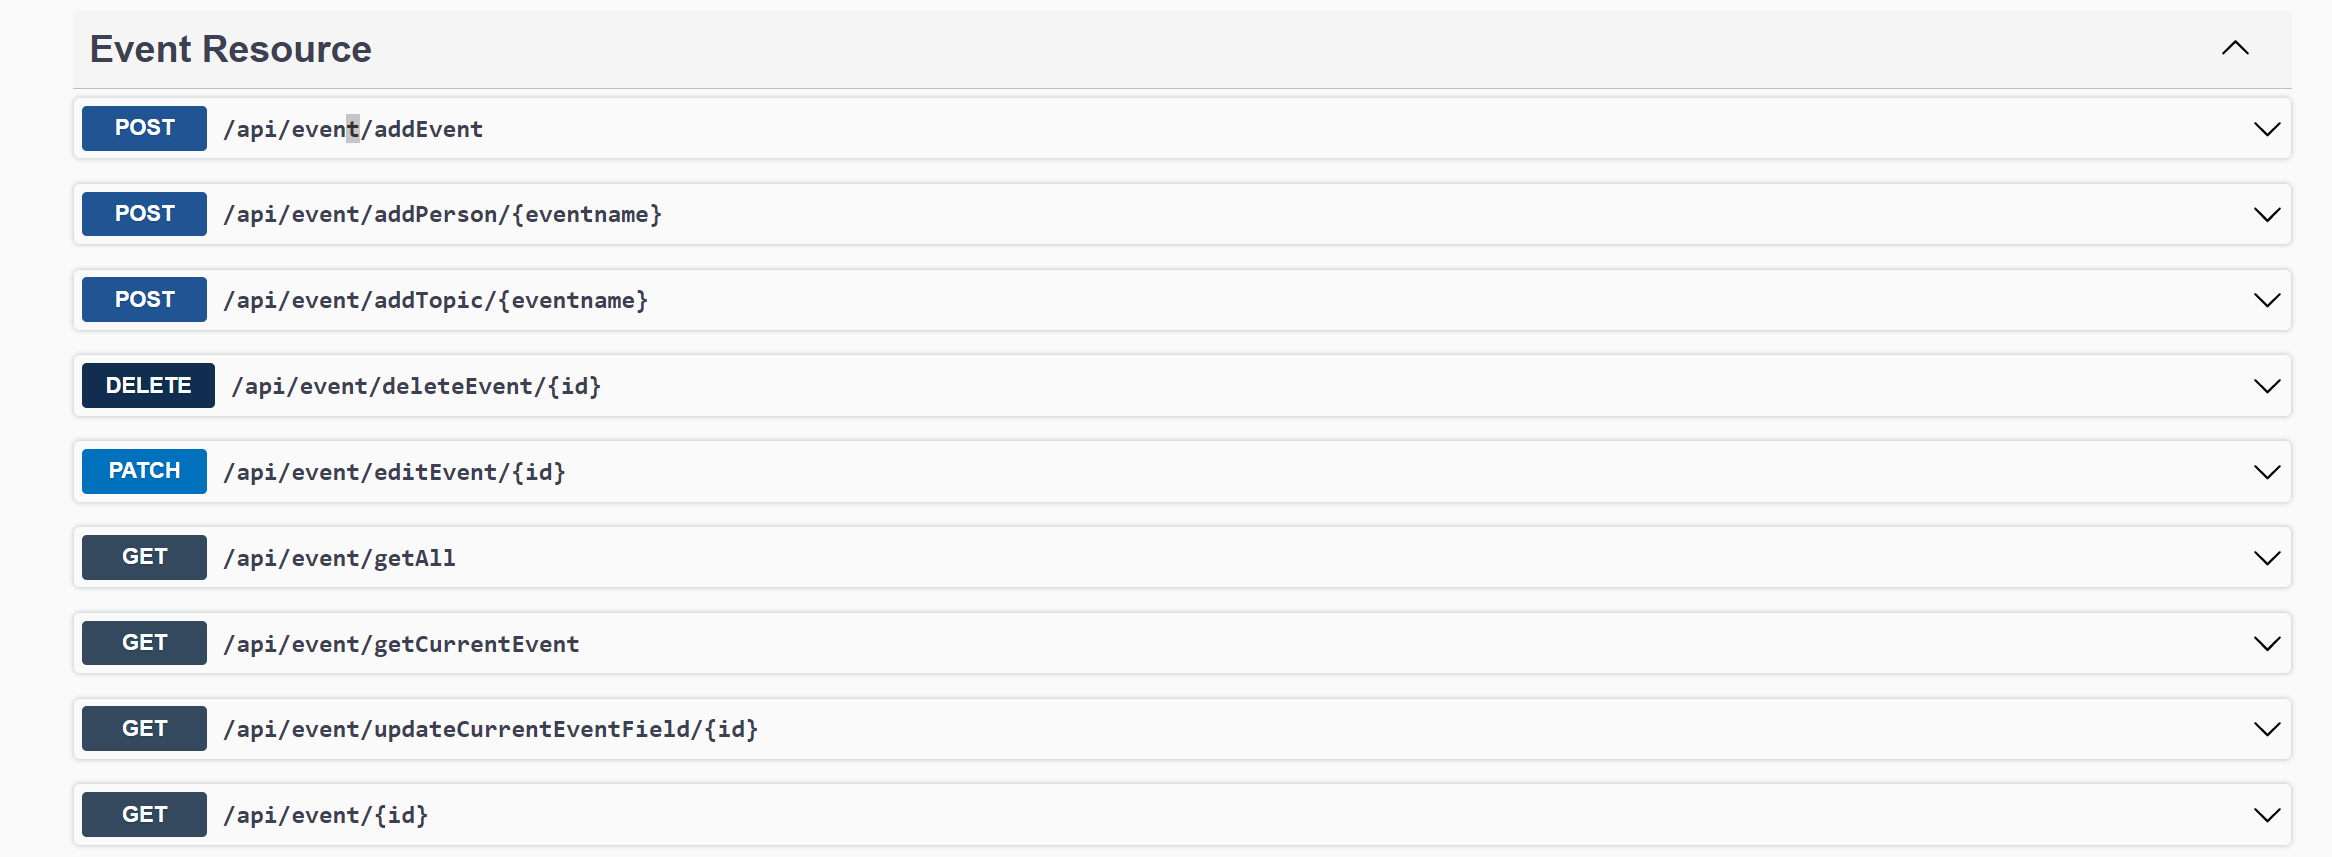
\includegraphics[scale=0.3]{pics/event_resource.png}
    \caption{Event Resource}
    \label{lst:event_resource}
\end{figure}

\begin{figure}[h]
    \centering
    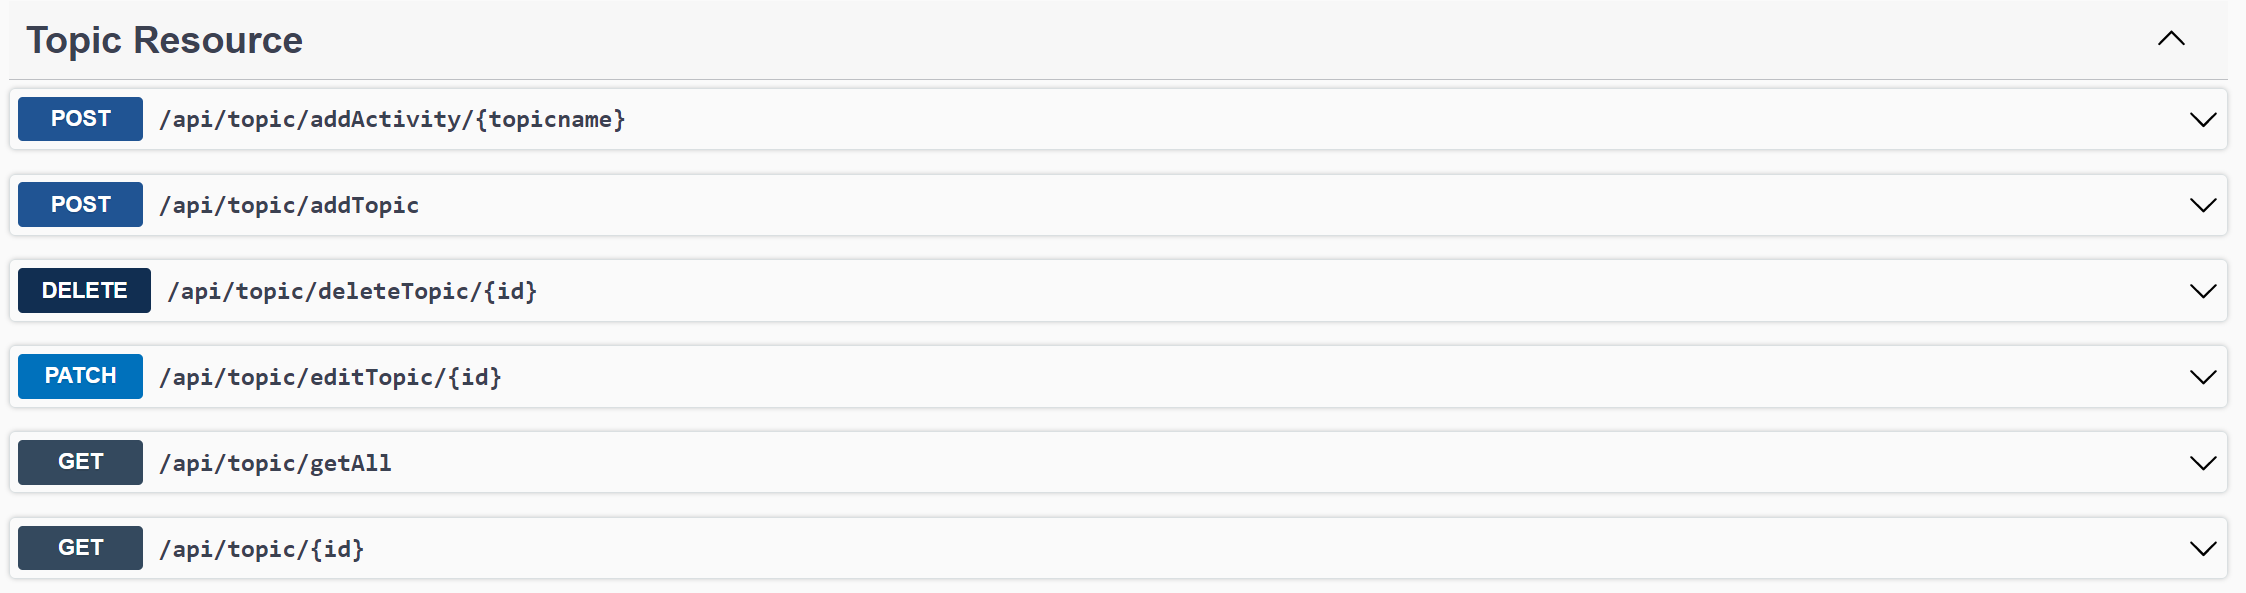
\includegraphics[scale=0.3]{pics/topic_resource.png}
    \caption{Topic Resource}    
    \label{lst:topic_resource}
\end{figure}

\begin{figure}[h]
    \centering
    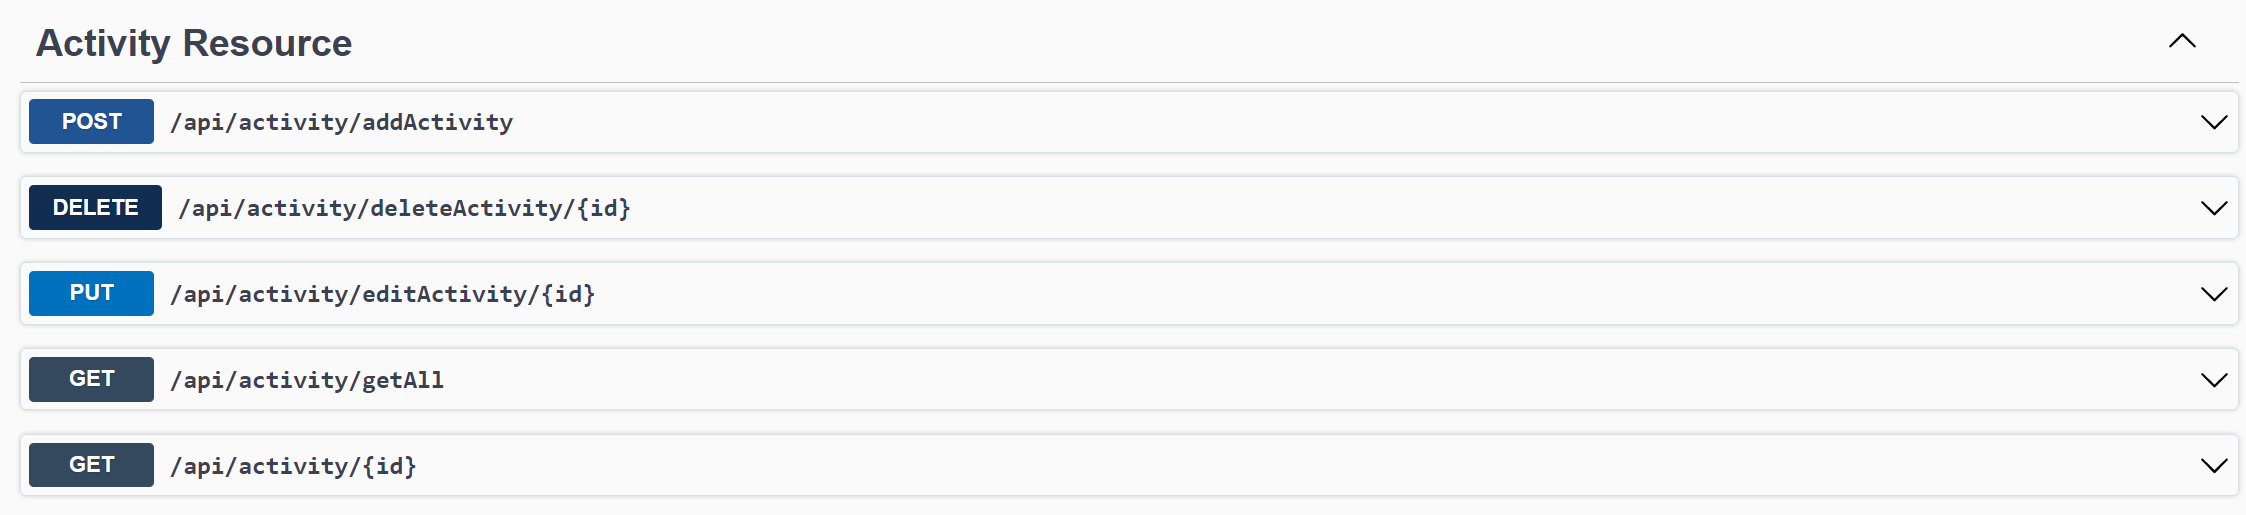
\includegraphics[scale=0.3]{pics/activity_resource.png}
    \caption{Activity Resource}
    \label{lst:activity_resource}
\end{figure}

\begin{figure}[h]
    \centering
    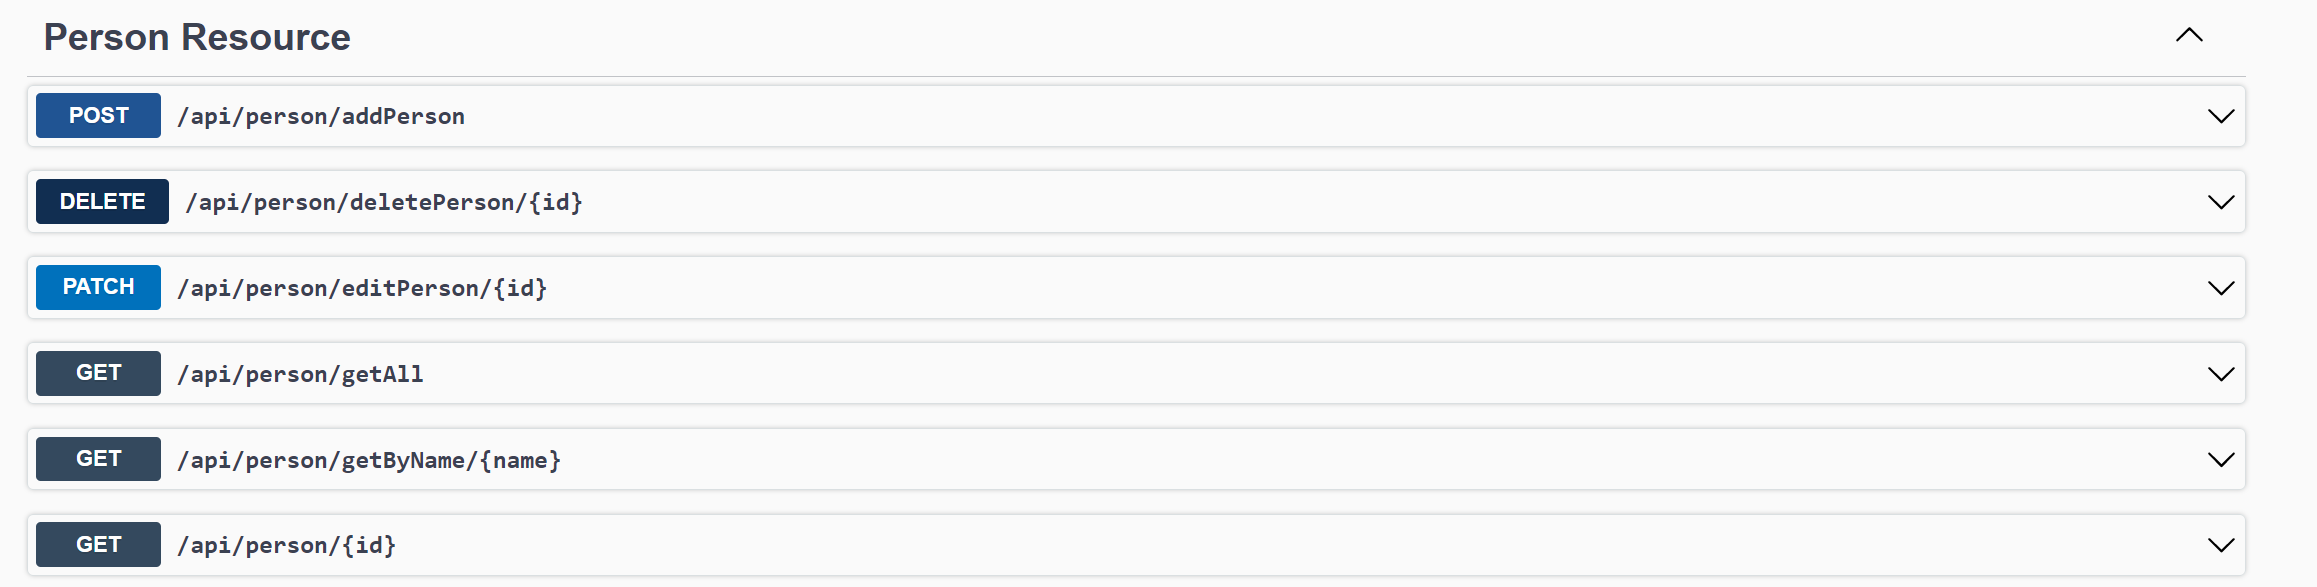
\includegraphics[scale=0.3]{pics/person_resource.png}
    \caption{Person Resource}
    \label{lst:person_resource}
\end{figure}

\subsection{Create Event}
\setauthor{Oliver Sugic}
 Wenn die Lehrerin oder Lehrer die Reise richtig angelegt haben, muss die  Struktur als JSON Objekt folgendermaßen aussehen:

\begin{lstlisting}[numbers=left, label={lst:json_post}]
{
    "location": "string",
    "maxPersonAllowed": 0,
    "type": "string",
    "participant": [
        {
        "firstname": "string",
        "lastname": "string",
        "role": "IN_CHARGE",
        "telephone": "string",
        "comment": "string",
        "event": "string"
        }
    ],
    "topics": [
        {
        "name": "string",
        "activity": [
            {
            "activityName": "string",
            "startDateTime": "2023-03-30T17:59:13.428Z",
            "longitude": 0,
            "latitude": 0,
            "previousActivity": "string",
            "comment": "string",
            "isPublic": true,
            "publicationDate": "2023-03-30",
            "topic": "string",
            "public": true
            }
        ],
        "previousTopic": "string",
        "event": "string",
        "comment": "string"
        }
    ],
    "planedStartDateTime": "2023-03-30T17:59",
    "planedEndDateTime": "2023-03-30T17:59",
    "currentEvent": true
}
\end{lstlisting}


\newpage

\subsection{Get Current Event}
\setauthor{Oliver Sugic}

Diese Methode wurde implementiert, um die aktuelle Reise zu bekommen. Die Methode gibt ein JSON Objekt zurück, welches die aktuelle Reise enthält. So kann man im Dashboard als auch in der Anzeige die aktuelle Reise anzeigen. Sie sieht wie folgt aus:


\begin{lstlisting}[numbers=left, label={lst:json_gte_by_id}]
    {
        "id": 1,
        "location": " Norditalien",
        "maxPersonAllowed": 100,
        "type": "Kulturwoche",
        "participant": [
            {
            "id": 1,
            "firstname": "Oliver",
            "lastname": "Sugic",
            "role": "STAFF",
            "telephone": "0123456789",
            "comment": "No comment"
            }
        ],
        "topics": [
            {
            "id": 1,
            "name": "Mailand",
            "activity": [
                {
                "id": 2,
                "activityName": "Koeniglicher Palast ",
                "startDateTime": "2023-05-11T16:00:00",
                "longitude": 9.1911,
                "latitude": 45.4632,
                "previousActivity": {
                    "id": 1,
                    "activityName": "Maeilaender Dom",
                    "startDateTime": "2023-05-11T13:00:00",
                    "longitude": 9.191926,
                    "latitude": 45.464098,
                    "previousActivity": null,
                    "comment": "Die Liste ..",
                    "publicationDate": "2023-03-30",
                    "public": true
                },
                "comment": "Kunstinteressierte s..",
                "publicationDate": "2023-03-30",
                "public": false
                }
            ],
            "previousTopic": null,
            "comment": "Mailand ist .."
            }
        ],
        "planedStartDateTime": "2022-05-19T09:30:00",
        "planedEndDateTime": "2023-05-15T00:00:00",
        "currentEvent": true
        }
\end{lstlisting}

Die Kommentare zu den jeweiligen Entitäten wurden gekürzt, um die Übersichtlichkeit zu gewährleisten.

\newpage

\subsection{List All Events}
\setauthor{Oliver Sugic}

Für die Liste aller Reisen nutze man \textbf{GET http://localhost:8080/api/event/getAll} Request. Die Methode gibt ein JSON Array zurück, welches alle Reisen enthält. Die Struktur sieht wie folgt aus:

\begin{lstlisting}[numbers=left, label={lst:json_gte_by_id}]
[{
    "id": 1,
    "location": " Norditalien",
    "maxPersonAllowed": 100,
    "type": "Kulturwoche",
    "participant": [
        {
        "id": 1,
        "firstname": "Oliver",
        "lastname": "Sugic",
        "role": "STAFF",
        "telephone": "0123456789",
        "comment": "No comment"
        }
    ],
    "topics": [
    ],
    "planedStartDateTime": "2022-05-19T09:30:00",
    "planedEndDateTime": "2023-05-15T00:00:00",
    "currentEvent": true
    },
    {
    "id": 2,
    "location": " Norditalien",
    "maxPersonAllowed": 100,
    "type": "Kulturwoche",
    "participant": [
        {
        "id": 1,
        "firstname": "Max",
        "lastname": "Musterman",
        "role": "STAFF",
        "telephone": "0123456789",
        "comment": "No comment"
        }
    ],
    "topics": [
    ],
    "planedStartDateTime": "2022-05-19T09:30:00",
    "planedEndDateTime": "2023-05-15T00:00:00",
    "currentEvent": false
}]
\end{lstlisting}

Die Topic Entitäten sind hier herausgekürzt worden, da sie in dem Kontext nicht relevant sind.


Die Reisen werde hier im Dashboard sichtbar angezeigt.

\begin{figure}[h]
    \centering
    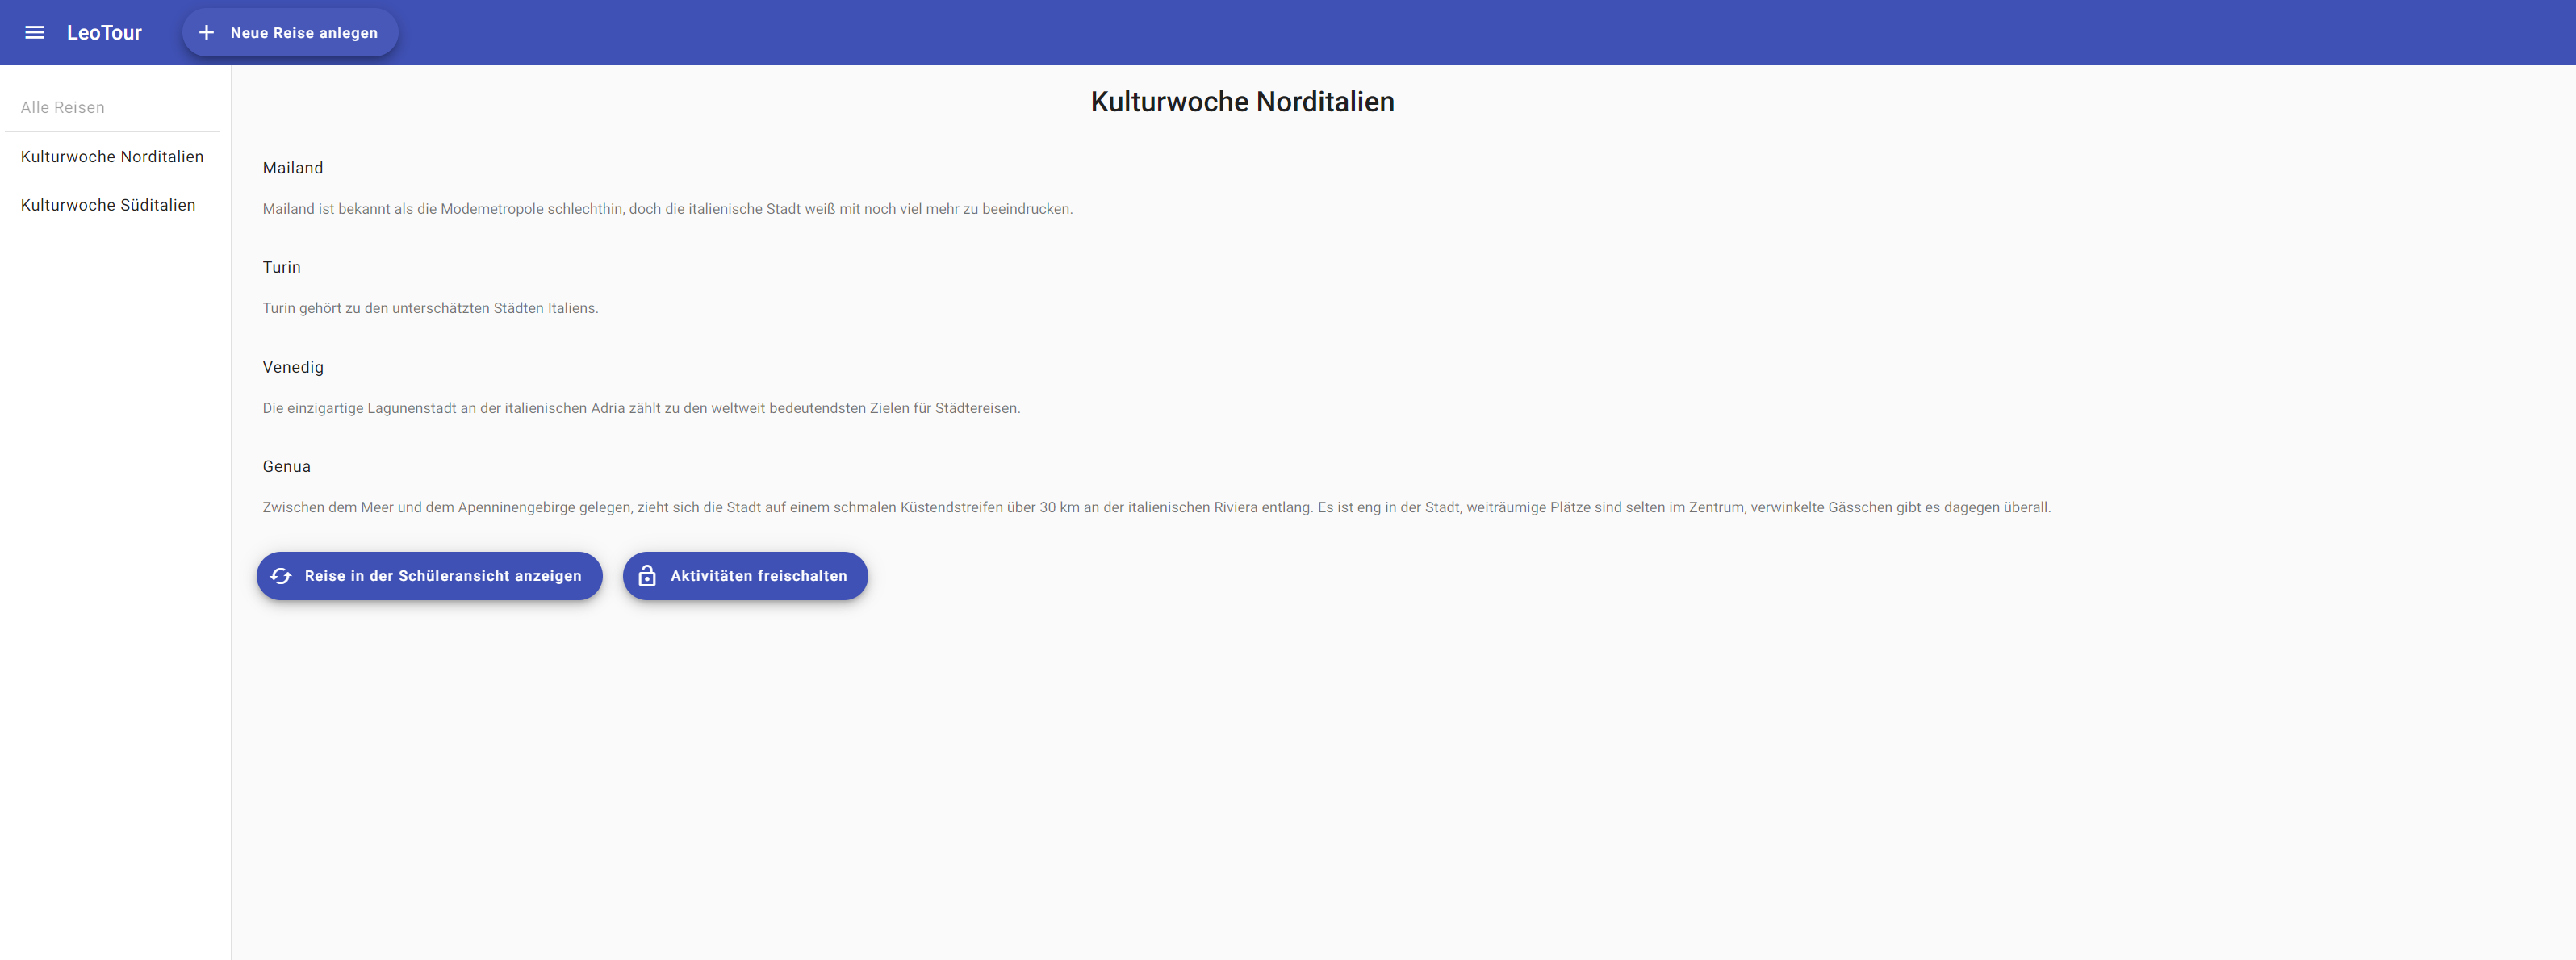
\includegraphics[scale=0.2]{pics/dashboard.png}
    \caption{Get All Example}
    \label{lst:list_all_Example}
\end{figure}    

